% --- SECCIÓ 1: INTRODUCCIÓ ---
\apartat{Introducció i Motivació}

\subsection{Motius de la tria del projecte}
La comunicació és un dret fonamental de tot ésser humà. No obstant això, per a moltes persones, aquest procés que la majoria realitzem de manera instintiva es converteix en una barrera infranquejable. La motivació principal d'aquest treball neix de la voluntat d'entendre i mitigar la frustració que senten aquelles persones que tenen idees, desitjos i emocions, però que no disposen dels canals adequats per expressar-los.

A nivell personal, l'interès neix d'observar com petits canvis en l'entorn poden transformar completament la interacció d'una persona amb el seu món. La taula sensorial és una eina que, tot i la seva aparent simplicitat física, amaga una gran complexitat de disseny pedagògic i terapèutic.

\begin{figure}[ht]
    \centering
    \begin{tcolorbox}[colback=white, colframe=MidnightBlue!20, arc=5pt, boxrule=0.5pt, left=2pt, right=2pt, top=2pt, bottom=2pt, shadow={1pt}{-1pt}{0pt}{black!5}]
        \centering
        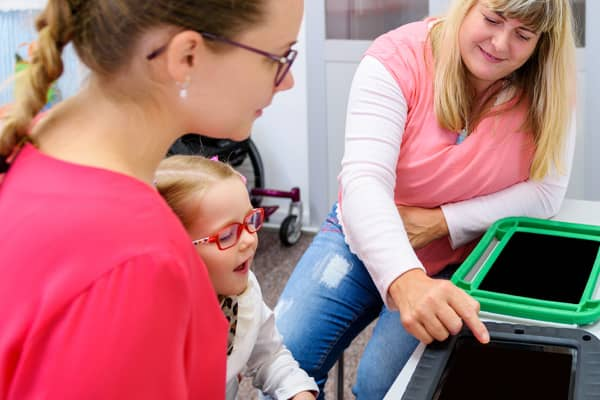
\includegraphics[width=0.8\textwidth]{imatges/persona-adulta-ensenyant-la-taula-de-neuroKids-per-la-communicacio-no-verbal-a-una-jove-i-una-nena-petita.jpg}
    \end{tcolorbox}
    \caption{Interacció multisensorial: l'espai com a facilitador de vincles afectius i aprenentatge social.}
    \label{fig:interaccio_sensorial}
\end{figure}

\newpage
\subsection{Orientació i objectius del treball}
Aquest projecte s'orienta des d'una perspectiva holística\footnote{Enfocament que considera la persona com un tot, integrant aspectes físics, psicològics i socials.}. L'enfocament es divideix en quatre eixos:
\begin{itemize}
    \item \textbf{Inclusió real:} Creació d'entorns accessibles per a tothom, potenciant l'autodeterminació\footnote{Capacitat de la persona per ser l'agent causal de la seva pròpia vida i prendre decisions sense influències externes indegudes.}.
    \item \textbf{Perspectiva logopèdica:} Reforç de les estructures del llenguatge mitjançant estímuls paral·lels.
    \item \textbf{Educació especial:} Proposta de materials tangibles per al suport a l'aula.
    \item \textbf{Impacte en la vida diària:} Solucions pràctiques per a l'entorn familiar.
\end{itemize}

\subsection{La importància de la diversitat en la societat actual}
Vivim en un món que a poc a poc va entenent que la diversitat no és un problema a resoldre, sinó un valor a integrar. Malgrat aquest avanç, encara trobem "deserts comunicatius"\footnote{Entorns on les persones amb dificultats no troben cap suport ni interlocutor preparat per entendre els seus mètodes alternatius de comunicació.} que cal abordar des de la innovació i el disseny inclusiu.
